\section{Results}
\label{sec:org28f7420}
So far, in sections \ref{sec:Analysis_method1} and \ref{sec:Analysis_method2}, we have studied how does a multivariate and a singlevariate calssifcation technique responds to energy scale uncertainties, in a signal from background sepparation task. In this chapter, we are going to summarize the results and provide commentary regarding each method, in terms of performance and robustness. Moreover will will draw a comparizon between the two methods.

\begin{figure}[htbp]
\centering
\includegraphics[page=4,width=0.5\textwidth]{/home/kpapad/UG_thesis/Thesis/Bdt/src/WPhiJets_M200M100300_Significance.pdf}
\caption{ Comparison of the perfomance of the BDT and Fit based analysis, in terms of sifnificance,  as a function of the smearing cases. We can see that BDT based analysis, is more robust.}
\label{fig:BdtFitSig}
\end{figure}

Figure \ref{fig:BdtFitSig}, compares the significance yielded by each method, as a function of smearing. 
Even though, at \(0\%\) of smearing, the fit based method, yields a better significance than the BDT method, the bdt is more robust in general. To explain this, on must pay close attention to the feature space used for the training. The classifier learns not only the energy related Pts of the X particles, but also the geometrical features, \(\Delta\phi\text{, }\Delta R\text{ and }\Delta\eta\). As discribed in section \ref{sec:Energy_scale_uncertainties}, smearing has an effect only on the Pt variables, while the spatial features remain invariant under such process. That is, the BDT model, learns to classify the signal, using features that do not change through out the smearing process, and is therefore able to deliver a better performance, when compared to the fit based analysis, which only makes use of the invariant mass, a feature that gets heavilly altered by uncertainties on the energy scale as figures \ref{fig:fits} and \ref{fig:extremeSmearings} indicate. 
